% \section{Implementation}

\subsection{Implementation and Evaluation Setup}
\begin{figure}
    \centering
    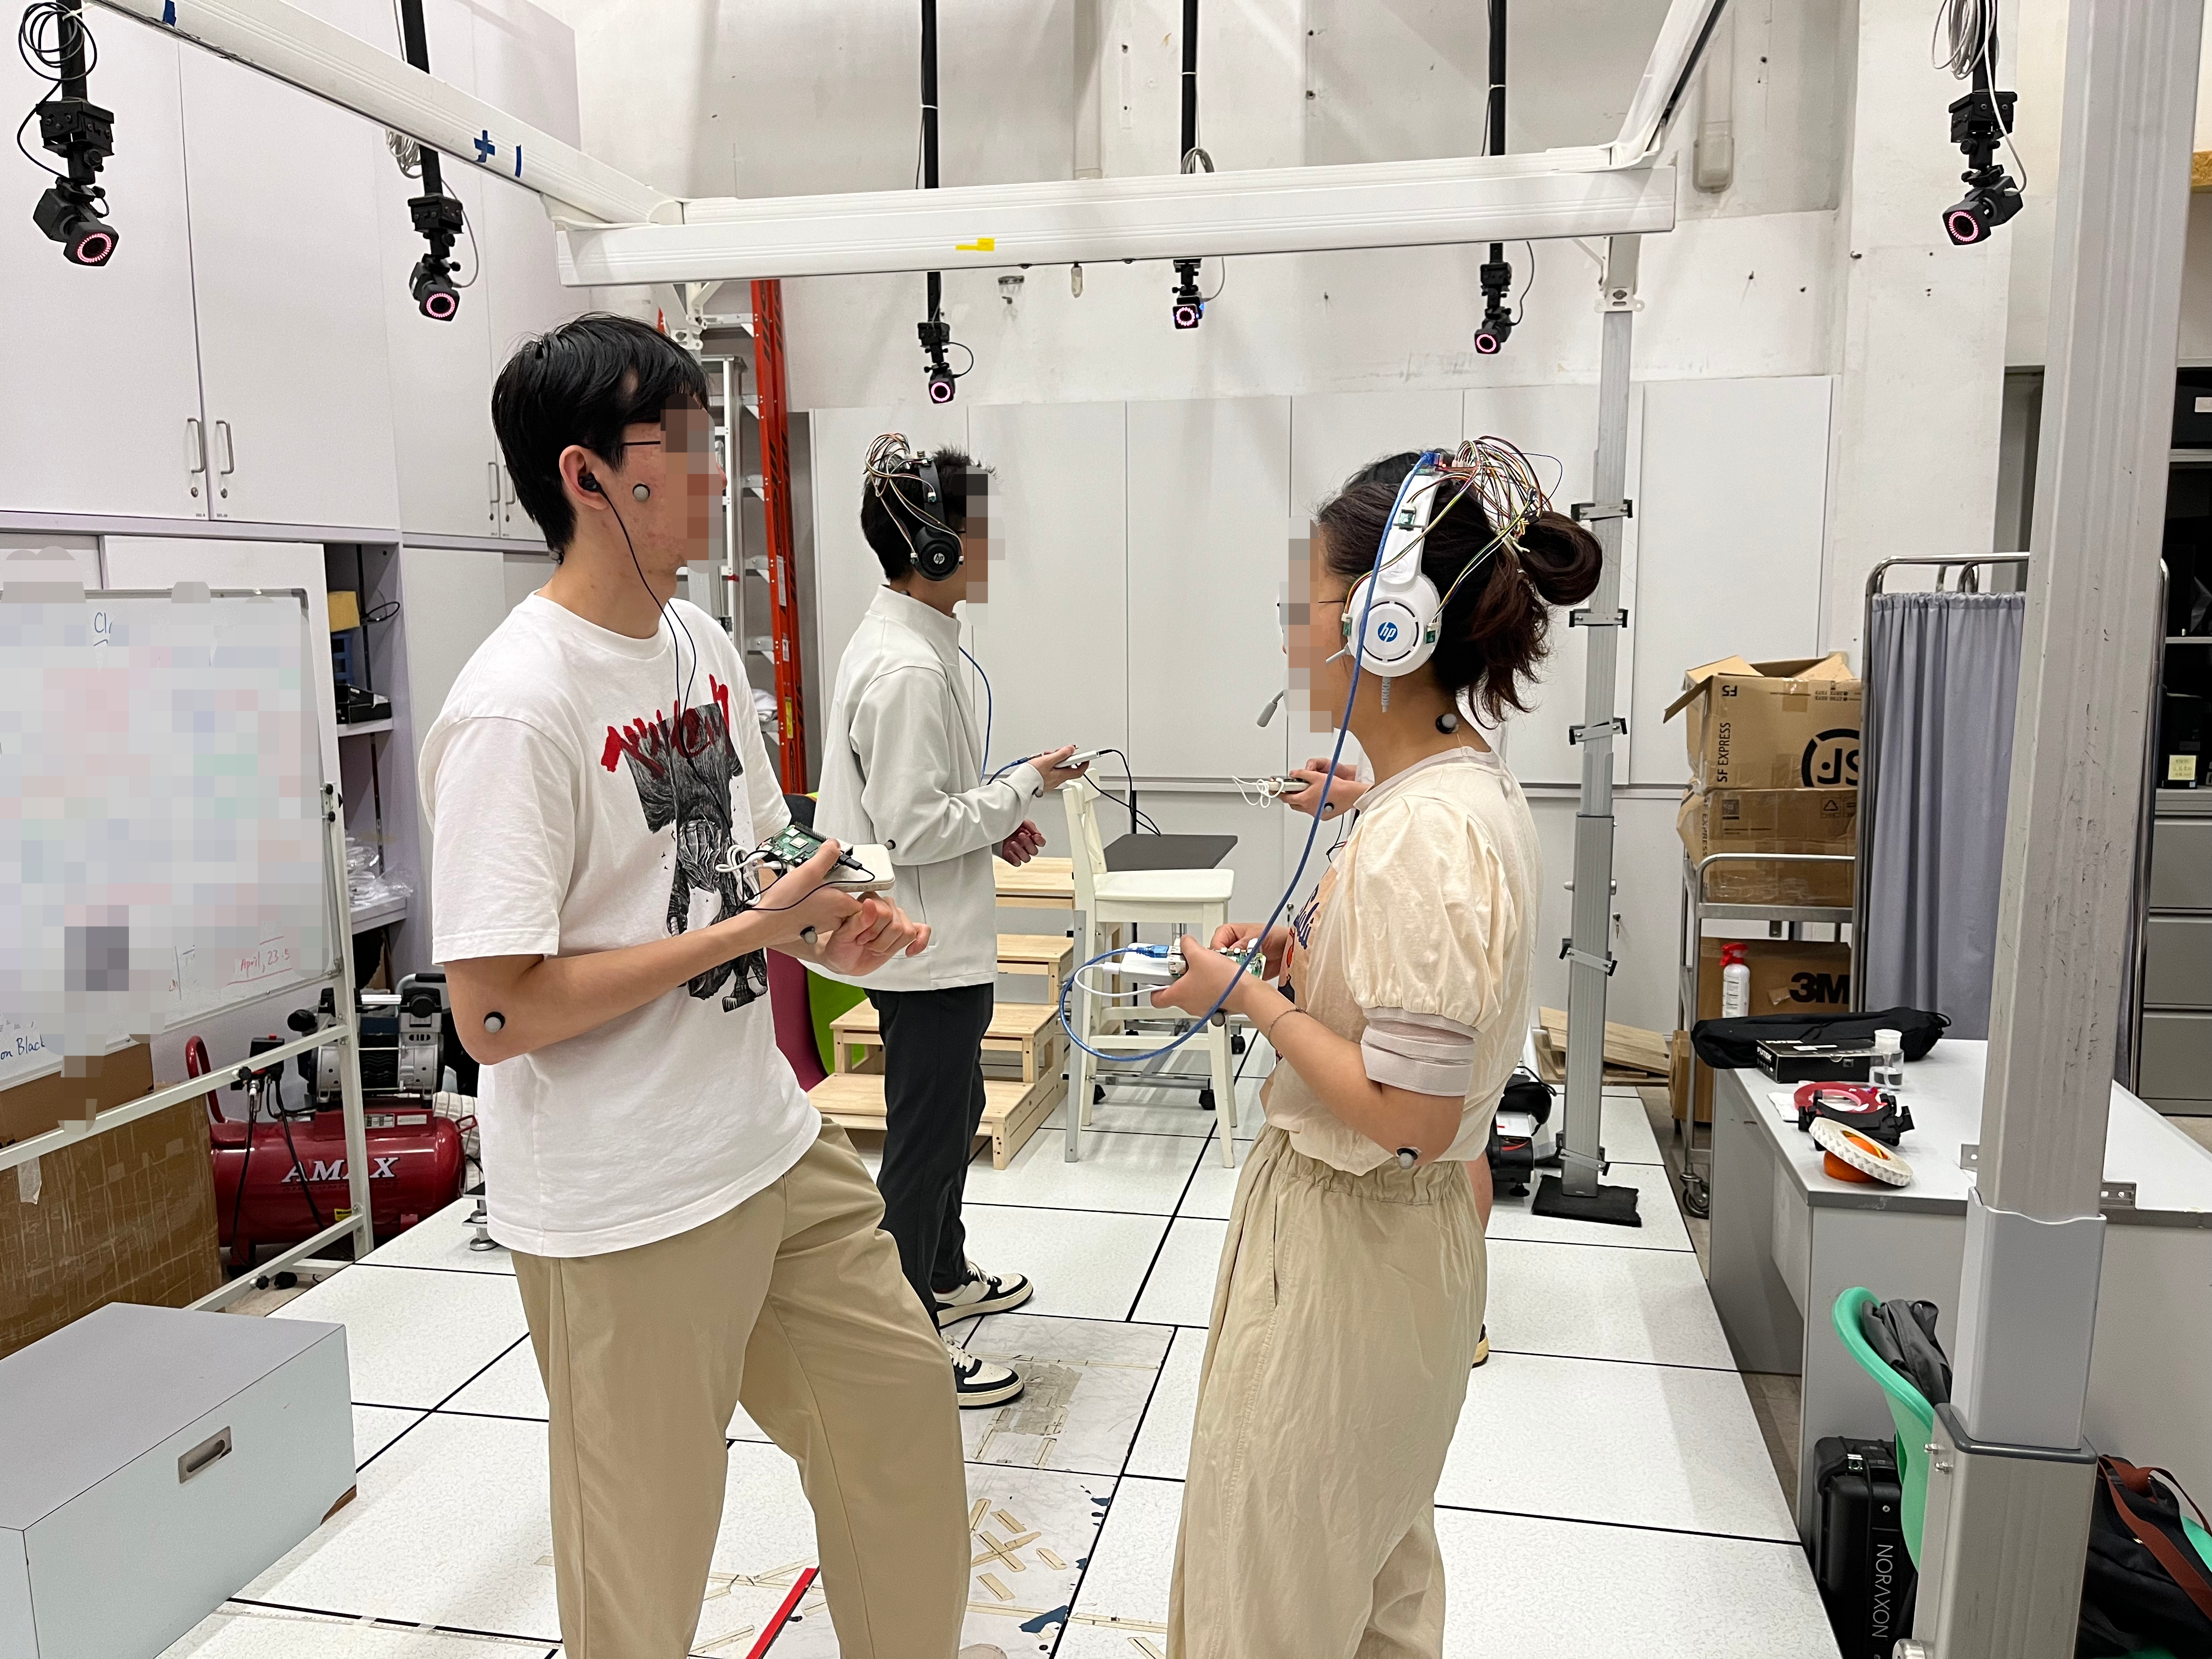
\includegraphics[width=0.5 \linewidth]{chapters/cohear/figs/experiment.png}
    \caption{Experiment setup of the motion capture room.}
    \label{fig:mocap}
    \vspace{-1em}
\end{figure}


\paragraph{Testbed Setup}
\label{sec:cohear_hardware}
We implement CoHear in various form factors, including binaural earphones and headphones with up to an 8-channel microphone array (placement is illustrated in Fig. \ref{fig:mic_loc}). The two earphones are shown in Fig. \ref{fig:hardware}. We use a Raspberry Pi 5 to collect audio and attach one IMU (BMI-160) to the headphones to track head motion, transmitted via I2C. For experimental validation, we connect each device via SSH under the same WiFi network, streaming all data to a desktop for analysis. The system output is designed to be played back through the headphone speakers, maintaining compatibility with existing ANC functionality. 

While our hardware supports sampling rates up to 48 kHz for maximum capture capability, the system is designed to operate at lower rates suitable for real-world deployment.
For practical speech applications, CoHear can operate at 8 kHz with audio compression to minimize bandwidth requirements, which is also evaluated in the later section.
Moreover, CoHear supports time-invariant speaker embeddings that require only one-time transmission, significantly reducing data size to 8192 bits in total, which is practical on even constrained networks. We also discuss the networking issue in Sec. \ref{sec:cohear_discuss}.


\begin{figure}[t]
    \centering
    \begin{minipage}{0.48\linewidth}
    \centering
    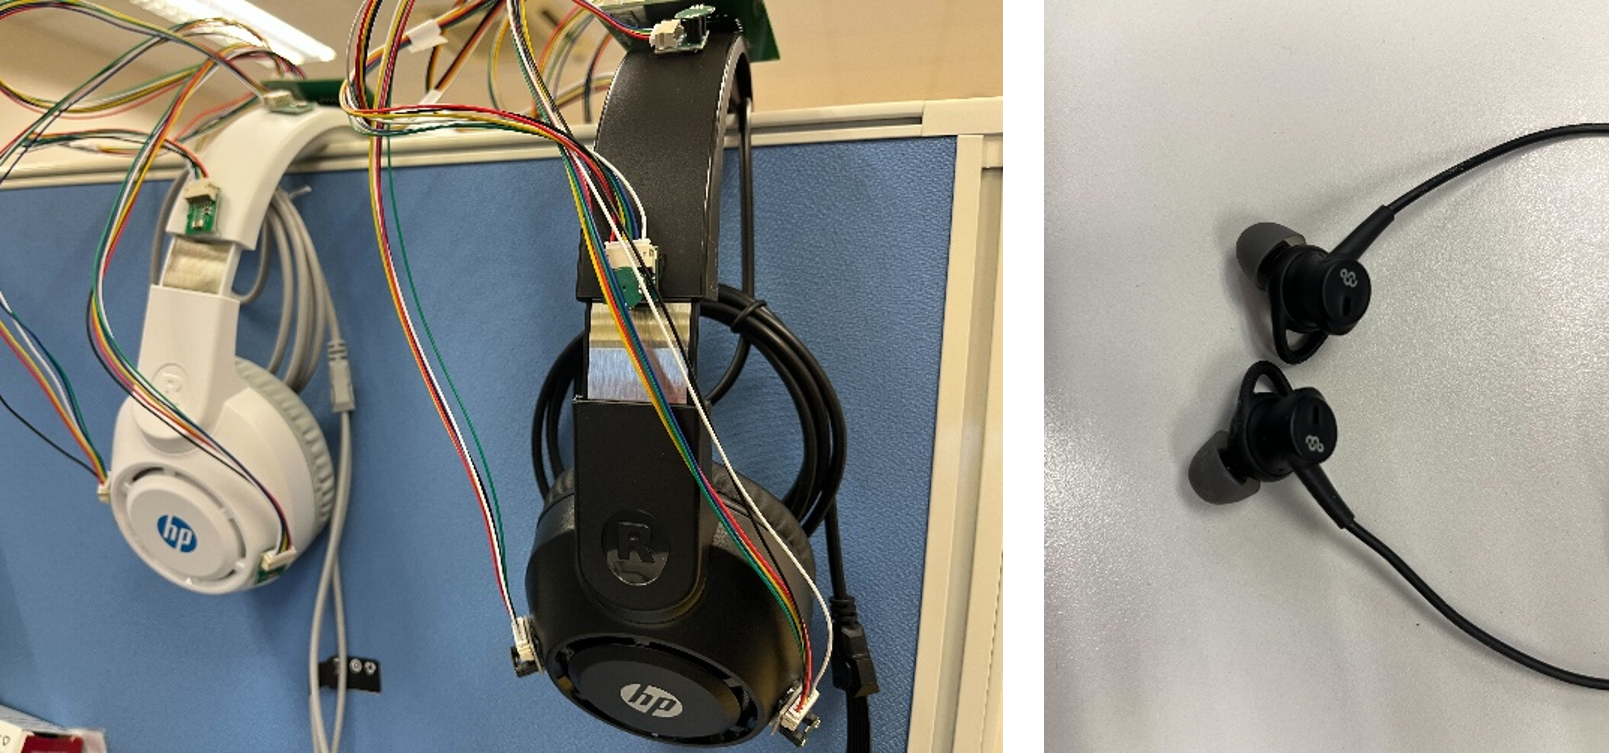
\includegraphics[width=0.8\linewidth]{chapters/cohear/figs/device.png}
    \caption{Hardware used in the experiment.}
    \label{fig:hardware}
    \end{minipage}
    \hfill
     \begin{minipage}{0.48\linewidth}
        \centering
        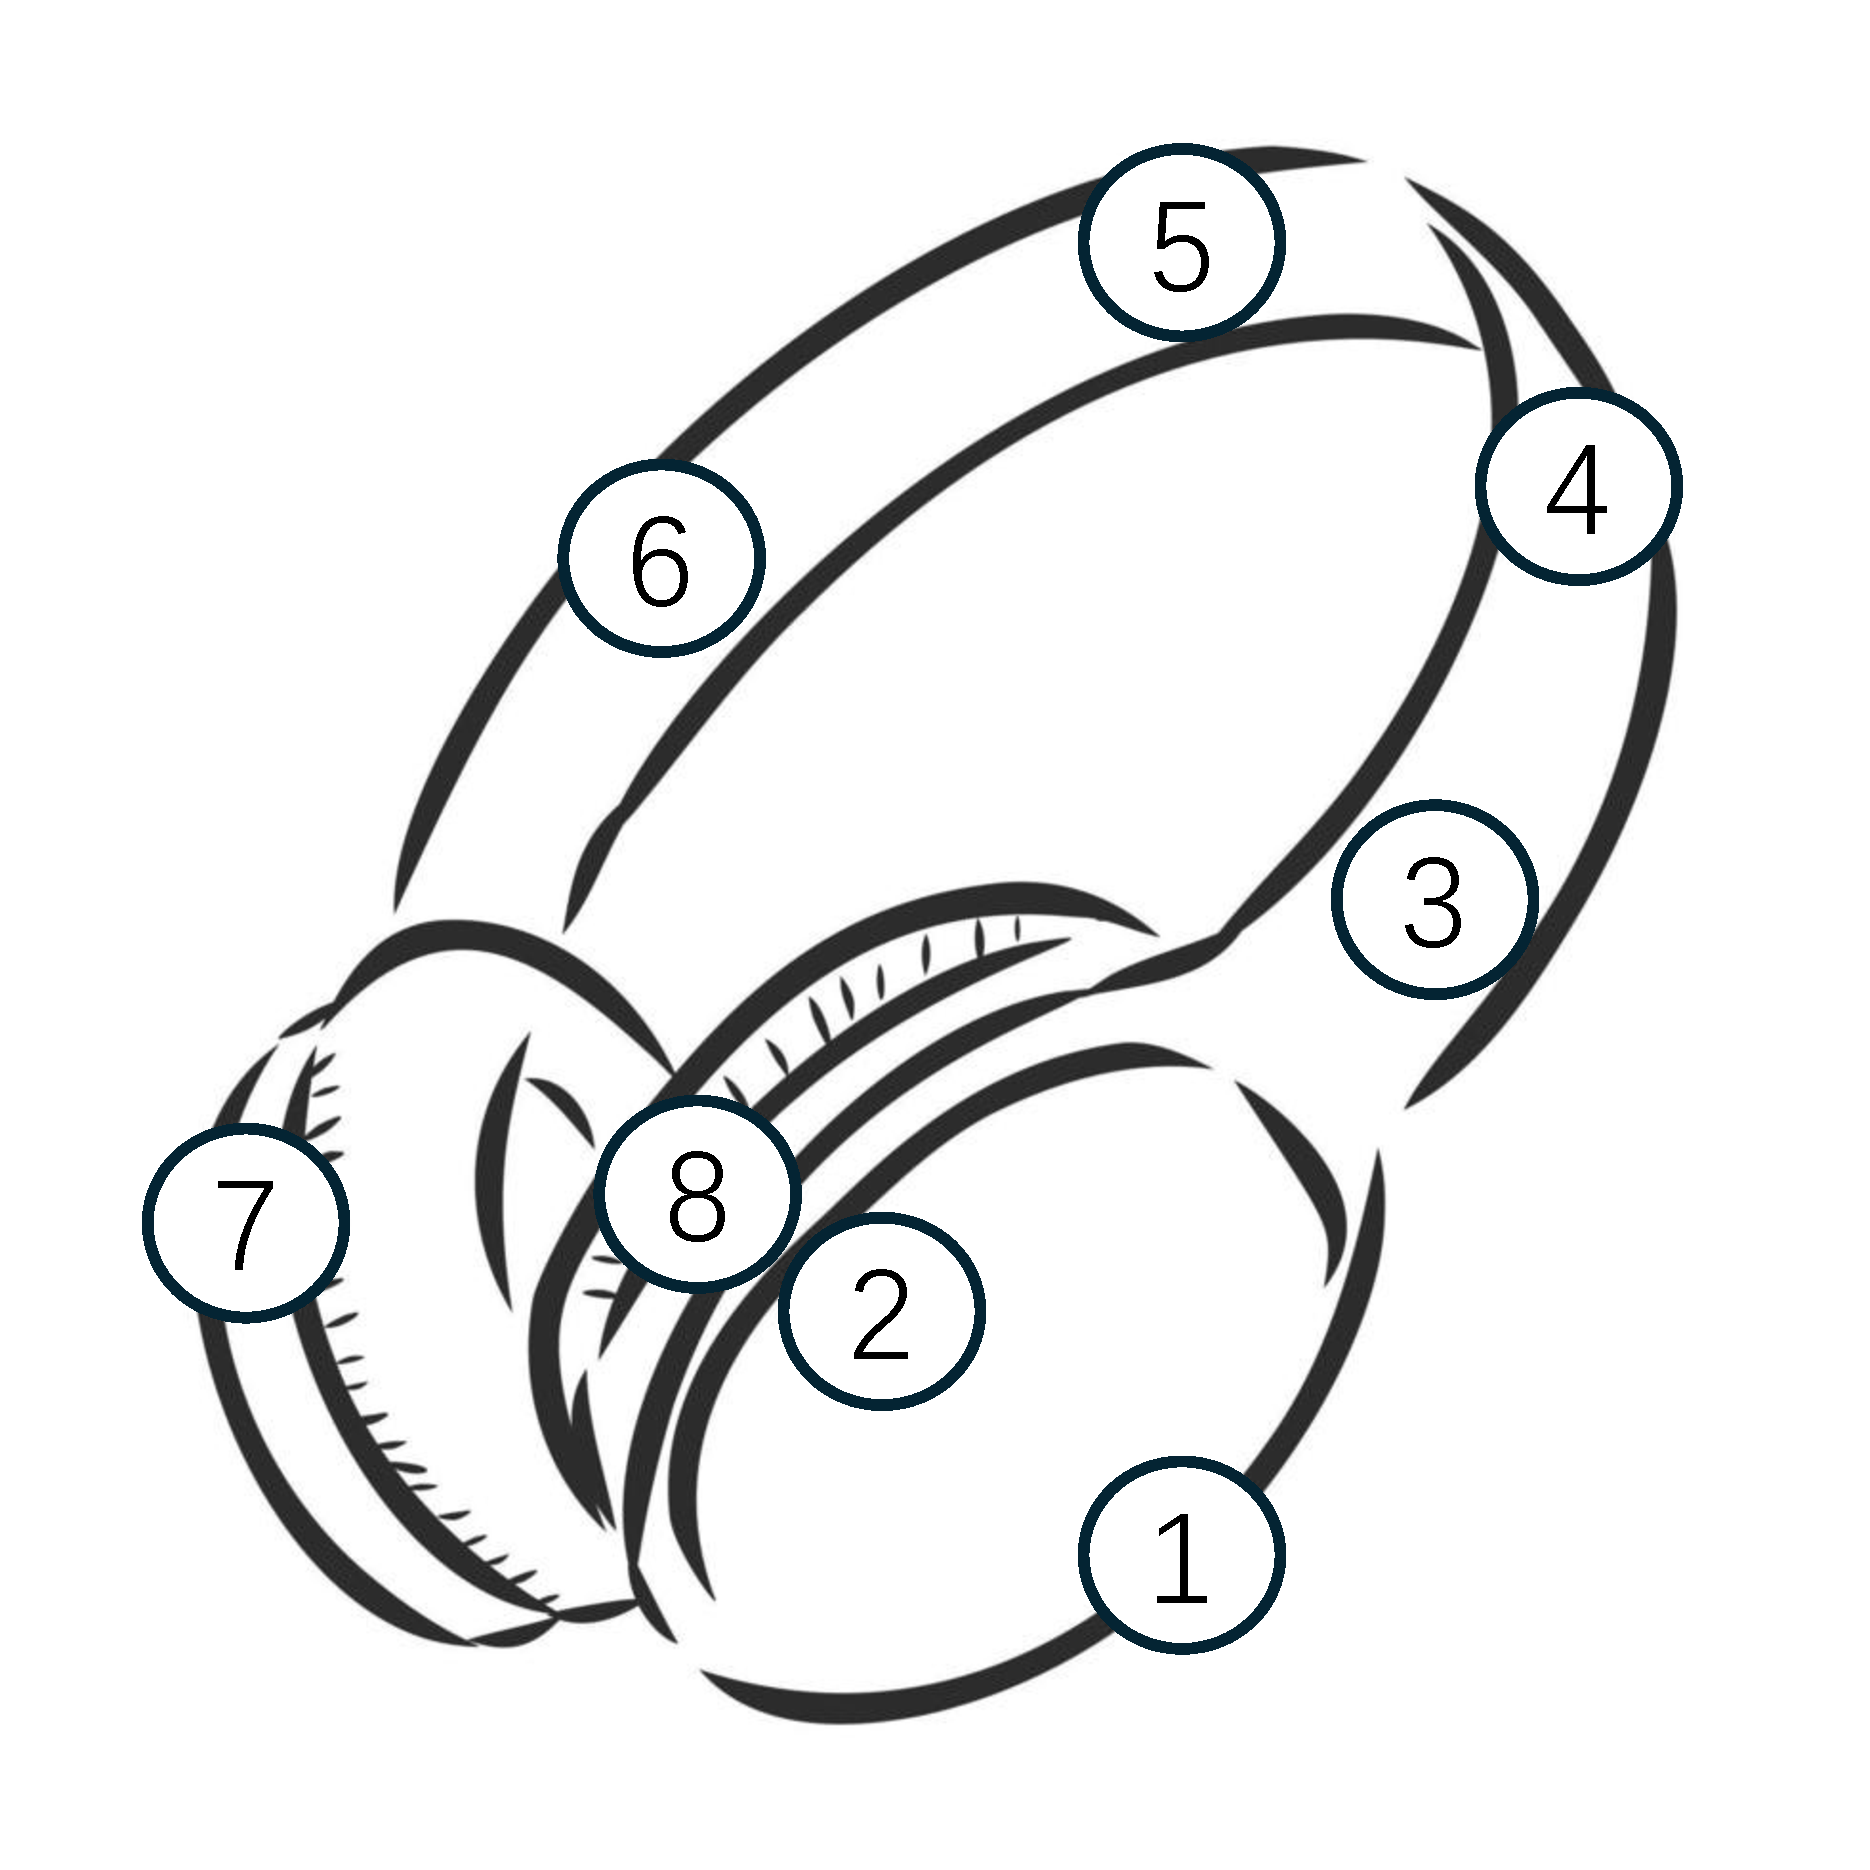
\includegraphics[width=0.4\linewidth]{chapters/cohear/figs/mic_loc.pdf}
    \caption{Microphones location on the headphone.}
    \label{fig:mic_loc}
    \end{minipage}%
    \vspace{-1em}
\end{figure}


\paragraph{Dataset Collection}
We use three data sources to support the design and evaluation of CoHear: a real-world dataset collected in a motion capture room, simulated datasets for large-scale testing and training, and public datasets for comparison.

\vspace{1ex}
\noindent\textit{Real-world Collection:}
We collected 30 minutes of multi-person conversation data in a $10 \times 5$ m motion capture room equipped with a 12-camera VICON system (Fig.~\ref{fig:mocap}). Markers were placed on participants’ heads and upper bodies to track conversational poses. Six volunteers wore our prototype headphones (Section~\ref{sec:cohear_hardware}) and engaged in natural turn-taking conversations. Due to space limitations, each session involved 2–4 participants in different grouping scenarios:
1) two participants in one group,
2) three participants with one excluded, and
3) four participants split into two groups.

\vspace{1ex}
\noindent\textit{Simulation:}
To scale beyond the limits of physical collection, we simulate two datasets: 1) Geometric Calibration: Using Pyroomacoustics~\cite{scheibler2018pyroomacoustics}, we simulate dynamic conversations in larger rooms (up to 20 m wide) with varied reverberation (RT60 from 0.25 to 0.75).
And 2) Conversation Extraction: We augment the real dataset with noisy-clean pairs and degraded relays (e.g., SNR, compression, bit crush, packet loss) to train and evaluate the enhancement model. The SNR of the noisy speech is set to between -10 dB and 10 dB.

\vspace{1ex}
\noindent\textit{Public Datasets:}
We also compare CoHear with existing datasets in Table~\ref{tab:comparison_dataset}. While prior work such as STARSS23~\cite{shimada2024starss23} and 6DoF-SELD~\cite{yasuda20246dof} focuses on sound event localization, and AMI~\cite{kraaij2005ami} and EasyCom~\cite{donley2021easycom} cover conversations, none support collaborative multi-device conversation modeling with 6DoF tracking as CoHear does.

\begin{table}[t]
\caption{Comparison with existing datasets.}
\centering
\begin{tabular}{|c|c|c|c|}
\hline
\textbf{Name} & \textbf{6DoF} & \textbf{Multi-device} & \textbf{Target} \\
\hline
STARSS23~\cite{shimada2024starss23} & No & No & Sound events \\
6DoF-SELD~\cite{yasuda20246dof} & Yes & No & Sound events \\
AMI~\cite{kraaij2005ami} & No & No & Conversation \\
EasyCom~\cite{donley2021easycom} & Yes & No & Conversation \\
\textbf{CoHear} & \textbf{Yes} & \textbf{Yes} & \textbf{Conversation} \\
\hline
\end{tabular}
\label{tab:comparison_dataset}
\end{table}



\paragraph{Evaluation Metrics}
The primary objectives of CoHear are to identify user locations and extract relevant conversations, assessed through distinct metrics.

For geometric calibration, we use two standard metrics: average direction error (in degrees) and location error (in meters). We also incorporate network setup accuracy, which indicates whether the participant can find the correct partner. Specifically, we define \(S_{i,j}\) equals to true if \(|R_{i,j} - O_i| < \frac{\pi}{4}\), where \(R_{i,j}\) is the relative direction from user \(j\) to user \(i\) and \(O_i\) is the orientation of user \(i\). 

As for the conversation enhancement, we will utilize the scale-invariant signal-to-noise ratio (Si-SNR) as a conversation-related metric, noting that the input SNR significantly influences results. Since the average default input SNR is set to 0 dB, allowing the output SNR to reflect improvements over the input.

\paragraph{Baselines Approaches}
Similar to the metrics, we also incorporate different baselines for the geometric calibration and conversation extraction, respectively.
For the former one, we consider \cite{gburrek2021geometry} as the baseline, which is designed for static WASN only. Besides, infrastructure-based acoustic localization \cite{gburrek2021geometry} and acoustic-SLAM \cite{evers2018acoustic} are related to CoHear. Note that when we apply \cite{gburrek2021geometry} as infrastructure-based acoustic localization, we have static nodes but mobile sources (i.e., users); our target becomes estimating the sound sources rather than nodes. We will use the following abbreviations in this paper: DSM refers to baseline \cite{gburrek2021geometry}, iDSM refers to infrastructure-based acoustic localization \cite{gburrek2021geometry}, and aSLAM for acoustic-SLAM \cite{evers2018acoustic}.


As for the conversation extraction, we consider LookOncetoHear \cite{veluri2024look}, target conversation extraction \cite{chen2024target}, and CoS \cite{jenrungrot2020cone} as our baselines. We also replace the relay audio with time-dependent speaker embedding as a baseline.
For LookOncetoHear \cite{veluri2024look}, we assume the enrollment happened in every sentence and takes effect in the next sentence. For the second baseline, we consider self-voice to be the condition. As for the CoS \cite{jenrungrot2020cone}, we assume the interferences span randomly in the nearby space while the target speaker is always in front of the user.
We will use the following abbreviations in this paper: LOTH stands for LookOnceToHear \cite{veluri2024look}, TC refers to \cite{chen2024target}, CoS refers to \cite{jenrungrot2020cone}

